\documentclass[english,a4paper,14pt,oneside]{extreport}

%%%%%%%%%%%%%%%%%%%%%%%%%%%%%%%%%%%%%%%%%%%%%%%%%%%%%%%%%%%%%%%%%%%%%%%%%%%%%%%
\usepackage{subcaption}
\usepackage[official]{eurosym}
\usepackage[dvips]{graphicx}
\usepackage[dvips]{epsfig}
\usepackage[utf8]{inputenc}
\usepackage{cite}
\usepackage{alltt}
\usepackage{multirow}
\usepackage{caption}
\usepackage{amsmath}
\usepackage{booktabs}
\usepackage{verbatim}
\usepackage[table,xcdraw]{xcolor}
\usepackage[toc,page]{appendix}
\usepackage{hyperref}
\hypersetup{
    colorlinks=true,
    linkcolor=black,
    filecolor=blue,      
    urlcolor=blue,
    citecolor=black
}
\usepackage{rotating,tabularx}
\usepackage{algorithm}
\floatname{algorithm}{Algorithm}
\usepackage[noend]{algpseudocode}
\usepackage{afterpage}
\usepackage{amsfonts}
\usepackage{xcolor}
\usepackage{capt-of}% or use the larger `caption` package
\usepackage{amstext} % for \text macro
\usepackage{array}   % for \newcolumntype macro
\newcolumntype{L}{>{$}l<{$}} % math-mode version of "l" column type
\usepackage[top=2cm, bottom=2cm, left=2cm, right=2cm]{geometry}

\usepackage{etoolbox,refcount}
\usepackage{multicol}
\newcounter{countitems}
\newcounter{nextitemizecount}
\newcommand{\setupcountitems}{%
  \stepcounter{nextitemizecount}%
  \setcounter{countitems}{0}%
  \preto\item{\stepcounter{countitems}}%
}
\makeatletter
\newcommand{\computecountitems}{%
  \edef\@currentlabel{\number\c@countitems}%
  \label{countitems@\number\numexpr\value{nextitemizecount}-1\relax}%
}
\newcommand{\nextitemizecount}{%
  \getrefnumber{countitems@\number\c@nextitemizecount}%
}
\newcommand{\previtemizecount}{%
  \getrefnumber{countitems@\number\numexpr\value{nextitemizecount}-1\relax}%
}
\makeatother    
\newenvironment{AutoMultiColItemize}{%
\ifnumcomp{\nextitemizecount}{>}{3}{\begin{multicols}{2}}{}%
\setupcountitems\begin{itemize}}%
{\end{itemize}%
\unskip\computecountitems\ifnumcomp{\previtemizecount}{>}{3}{\end{multicols}}{}}

%%%%%%%%%%%%%%%%%%%%%%%%%%%%%%%%%%%%%%%%%%%%%%%%%%%%%%%%%%%%%%%%%%%%%%%%%%%%%%%

%%%%%%%%%%%%%%%%% Creamos un entorno para listar código fuente %%%%%%%%%%%%%%%
\newenvironment{sourcecode}
{\begin{list}{}{\setlength{\leftmargin}{1em}}\item\scriptsize\bfseries}
{\end{list}}

\newenvironment{littlesourcecode}
{\begin{list}{}{\setlength{\leftmargin}{1em}}\item\tiny\bfseries}
{\end{list}}

\newenvironment{summary}
{\par\noindent\begin{center}\textbf{Abstract}\end{center}\begin{itshape}\par\noindent}
{\end{itshape}}

\newenvironment{keywords}
{\begin{list}{}{\setlength{\leftmargin}{1em}}\item[\hskip\labelsep \bfseries Keywords:]}
{\end{list}}

\newenvironment{palabrasClave}
{\begin{list}{}{\setlength{\leftmargin}{1em}}\item[\hskip\labelsep \bfseries Palabras clave:]}
{\end{list}}


%%%%%%%%%%%%%%%%%%%%%%%%%%%%%%%%%%%%%%%%%%%%%%%%%%%%%%%%%%%%%%%%%%%%%%%%%%%%%%%
% Format
%%%%%%%%%%%%%%%%%%%%%%%%%%%%%%%%%%%%%%%%%%%%%%%%%%%%%%%%%%%%%%%%%%%%%%%%%%%%%%%
%\usepackage{showframe}
%\marginparwidth 0mm
%%\topmargin -4 mm
%\topmargin -21 mm
%\headheight 10 mm
%\headsep 10 mm

%\textheight 229 mm
%\textheight 246 mm

%\oddsidemargin -5.4 mm
%\evensidemargin -5.4 mm
%\oddsidemargin 5 mm
%\evensidemargin 5 mm

%\oddsidemargin -3 mm
%\evensidemargin -3 mm

%\textwidth 17 cm
%\textwidth 15 cm
%\columnsep 10 mm

\input{amssym.def}

%%%%%%%%%%%%%%%%%%%%%%%%%%%%%%%%%%%%%%%%%%%%%%%%%%%%%%%%%%%%%%%%%%%%%%%%%%%%%%%

\begin{document}

%%%%%%%%%%%%%%%%%%%%%%%%%%%%%%%%%%%%%%%%%%%%%%%%%%%%%%%%%%%%%%%%%%%%%%%%%%%%%%%
% First Page
%%%%%%%%%%%%%%%%%%%%%%%%%%%%%%%%%%%%%%%%%%%%%%%%%%%%%%%%%%%%%%%%%%%%%%%%%%%%%%%

\pagestyle{empty}
\thispagestyle{empty}


\newcommand{\HRule}{\rule{\linewidth}{1mm}}
\setlength{\parindent}{0mm}
\setlength{\parskip}{0mm}

\vspace*{\stretch{0.5}}

\begin{center}

\includegraphics[scale=1.5]{images/marca.png}\\[10mm]
{\Huge Masters Degree Thesis}
\end{center}

\HRule
\begin{flushright}
        {\Huge On the healthy and balanced menu planning automatisation} \\[2.5mm]
        {\Large Planificación automática de menús saludables y equilibrados}\\[2.5mm]
        {\Large Alejandro Marrero Díaz} \\[5mm]


\end{flushright}
\HRule
\vspace*{\stretch{2}}
\begin{center}
  \Large La Laguna, XX March 2019
\end{center}

\setlength{\parindent}{5mm}

%%%%%%%%%%%%%%%%%%%%%%%%%%%%%%%%%%%%%%%%%%%%%%%%%%%%%%%%%%%%%%%%%%%%%%%%%%%%%%%
% Signature page (add the official stamp)
%%%%%%%%%%%%%%%%%%%%%%%%%%%%%%%%%%%%%%%%%%%%%%%%%%%%%%%%%%%%%%%%%%%%%%%%%%%%%%%
\newpage
%\cleardoublepage
\thispagestyle{empty}

Mr. {\bf Eduardo Manuel Segredo González}, con N.I.F. 78-564-242-Z
Part-time lecturer at Departamento 
de Ingeniería Informática y de Sistemas
de la Universidad de La Laguna, as mentor

\bigskip
Mrs. {\bf Coromoto Antonia León Hernández}, with N.I.F. 78-605-216-W
Full-time lecturer at Departamento 
de Ingeniería Informática y de Sistemas
de la Universidad de La Laguna, as mentor

\bigskip
\bigskip
{\bf C E R T I F Y}

\bigskip
\bigskip
\bigskip
That this report named:

\bigskip
``{\it On the healthy and balance menu planning automatisation.}''

\bigskip
\bigskip
\bigskip

\noindent has been done under they supervision by Mr. {\bf Alejandro Marrero Díaz},
with N.I.F. 78-649-404-F.

\bigskip
\bigskip

And to be recorded, in compliance of the current legislation and timely effects XX March 2019.

%\cleardoublepage
\newpage
%%%%%%%%%%%%%%%%%%%%%%%%%%%%%%%%%%%%%%%%%%%%%%%%%%%%%%%%%%%%%%%%%%%%%%%%%%%%%%%
\thispagestyle{empty}

{ \flushright

\begin{LARGE}
Acknowledgements 
\end{LARGE}

\hspace{3mm}

\begin{large}


\hspace{3mm}
%A mi familia y amigos que

\hspace{3mm}
%me han apoyado incondicionalmente estos cuatro años.

\bigskip

\hspace{3mm}
%Agradecer también a los directores de este Trabajo de Fin de Grado,

\hspace{3mm}
%Eduardo Segredo y Carlos Segura,

\hspace{3mm}
%por la ayuda en el desarrollo del mismo

\hspace{3mm}
%y por adentrarme en el mundo de la investigación.

\end{large}

}

%%%%%%%%%%%%%%%%%%%%%%%%%%%%%%%%%%%%%%%%%%%%%%%%%%%%%%%%%%%%%%%%%%%%%%%%%%%%%%%%%
\newpage

\begin{huge}
License
\end{huge}
\begin{center}

\includegraphics[scale=1.5]{images/by-nc-sa_88x31}\\[10mm]
{\Large \copyright~This work is under Creative Commons license.
}
\end{center}



%%%%%%%%%%%%%%%%%%%%%%%%%%%%%%%%%%%%%%%%%%%%%%%%%%%%%%%%%%%%%%%%%%%%%%%%%%%%%%%
\newpage  %\cleardoublepage

%%%%%%%%%%%%%%%%%%%%%%%%%%%%%%%%%%%%%%%%%%%%%%%%%%%%%%%%%%%%%%%%%%%%%%%%%%%%%%%
\newpage  %\cleardoublepage
\begin{abstract}
{\em

With the raise of diseases related with unhealthy lifestyles such as heart-attacks, overweight, diabetes, etc. Encouraging healthy and balanced patterns in the population is one of the most important action points for governments around the world. Furthermore, it is actually even a more critical situation when a high percentage of patients are child and teenagers whose habits consists merely in eating fast or ultra-processed food and a sedentary life.

The development of healthy and balanced menu plans became a routine task for physicians and nutritionists, and it is at this point that computer science has taken an important role. Discovering new approaches for generating healthy and balanced as well as inexpensive menu plans will play a part in banish of diseases from actual and new generations.

In this Master Thesis, a evolutionary algorithm have been compared with other state-of-art evolutionary algorithm for solving the Menu Planning Problem. In order to evaluate the performance of the developed algorithm, an exhaustive experimental research was made. Firstly, we focused on evaluate the parameter setting of the algorithm so afterwards the best configuration found could be compared with other algorithms. 
}

\begin{keywords}
menu-plan, computer-science
\end{keywords}

\end{abstract}

%%%%%%%%%%%%%%%%%%%%%%%%%%%%%%%%%%%%%%%%%%%%%%%%%%%%%%%%%%%%%%%%%%%%%%%%%%%%%%%
\newpage{\pagestyle{empty}}
\thispagestyle{empty}

%%%%%%%%%%%%%%%%%%%%%%%%%%%%%%%%%%%%%%%%%%%%%%%%%%%%%%%%%%%%%%%%%%%%%%%%%%%%%%%


\pagestyle{myheadings} %my head defined by markboth or markright
% No funciona bien \markboth sin "twoside" en \documentclass, pero al
% ponerlo se dan un montón de errores de underfull \vbox, con lo que no se
% ha puesto.
\markboth{Alejandro Marrero Díaz}{On the healthy and balance menu planning automatisation}

%%%%%%%%%%%%%%%%%%%%%%%%%%%%%%%%%%%%%%%%%%%%%%%%%%%%%%%%%%%%%%%%%%%%%%%%%%%%%%%
%Numeracion en romanos
\renewcommand{\thepage}{\roman{page}}
\setcounter{page}{1}

\tableofcontents
%%%%%%%%%%%%%%%%%%%%%%%%%%%%%%%%%%%%%%%%%%%%%%%%%%%%%%%%%%%%%%%%%%%%%%%%%%%%%%%
\newpage{\pagestyle{empty}}
\listoffigures
%%%%%%%%%%%%%%%%%%%%%%%%%%%%%%%%%%%%%%%%%%%%%%%%%%%%%%%%%%%%%%%%%%%%%%%%%%%%%%%
\newpage{\pagestyle{empty}}
\listoftables
%%%%%%%%%%%%%%%%%%%%%%%%%%%%%%%%%%%%%%%%%%%%%%%%%%%%%%%%%%%%%%%%%%%%%%%%%%%%%%%
\newpage{\pagestyle{empty}}

\chapter{Motivation}\label{ref:motivation}
\section{Description of the Master thesis}

\section{Antecedent and current status of the topic}
\newpage{\pagestyle{empty}}
\chapter{Introduction}\label{ref:intro}
\section{Optimisation Problems}
An Optimisation Problem~(OP) is a problem which has a score function and bounds where the main task is to find a input that optimises the score function. Optimisation problems can be categorised as \textit{discrete optimisation problem~(DOP)} or \textit{continuous optimisation problem~(COP)} whether the variables of the problem are discrete or continuous. 
Formally speaking, an OP can be described as follows:
\begin{equation*}
min\;f(x), x \in \chi,\quad s.t.\:\Omega
\end{equation*}
where $\chi \subset\mathbb{R}^{n}$ is the search space defined over a set of \textit{n} decision variables  $x = ~(x_{1}, x_{2},..., x_{n})$, $f: \chi \rightarrow \mathbb{R}$ is the score function and $\Omega$ is the restrictions set in $x$. This is the definition for a minimisation DOP, although it would be equivalent for a maximisation DOP changing $min\;f(x)$ by $max\;f(x)$. The same happens for a COP, if in addition the decision variables are set over $\mathbb{Z}^{n}$ instead of $\mathbb{R}^{n}$ .

Furthermore, optimisation problems may have more than one score function and they are called \textit{Multi-Objective Optimisation Problems~(MOOP)}. This is the primary field of study in this work so, hereinafter all the references to optimisation problems in this work will be to MOOP.
\newpage
\subsection{Multi-Objective Optimisation Problems}

Multi-Objective Optimisation Problems~(MOOPs) are for those kind of optimisation problems where there are  two or even more objective functions to optimise and those objective functions can take opposite directions (thinking about directions as \textit{minimise or maximise}). Besides, a MOOP can discrete or continuous considering whether the variables of the problem are discrete or continuous. \\
Formally speaking, a MOOP can be described as finding a vector \textbf{$x$} inside the problem's search space \textit{$\chi$} in such way that optimises the vector of objective functions \textit{$f(x)$}\cite{search}:
\begin{align*}
min\;f(x) & = (f_{1}(x), f_{2}(x), ..., f_{k}(x)), \: x\;\in\chi \\
 g_{i}(x) & \leq 0, \: i = 1, 2, ..., q. \\
 h_{i}(x) & \leq 0, \: i = 1, 2, ..., p.
\end{align*}
where $x = (x_{1}, x_{2}, ..., x_{n}) \in \mathbb{Z}^{n}$, are the objective functions to optimise $f_{i}: \mathbb{Z}^{n} \rightarrow \mathbb{R}, \; i = 1, ..., k$ being \textit{n} the number of decision variables and $g_{i}: \mathbb{Z}^{n} \rightarrow \mathbb{R}, \; i = ~1, ..., q$ and $h_{i}: \mathbb{Z}^{n} \rightarrow \mathbb{R}, \; i = 1, ..., p$ are the problem's restriction functions.

Moreover, the standard method for solving a MOOP is the well-known \textit{Pareto method}\cite{search}. The Pareto method is based on the non-dominance principle\cite{search, metaheuristics}. On the one hand, dominance means that given two solutions for a MOOP, one solutions dominates the other one when it has as least the same quality for every objective and, it has strictly more quality for one of them than the other solution. Formally, this can be expressed as follows\cite{search}:
\begin{align*}
A \succeq  B \Leftrightarrow & \forall i \in \{1, 2, ..., n\} \: a_{i} \leq b_{i}, \\
& y\;\exists i \in \{1, 2, ..., n\}, \: a_{i} < b_{i}
\end{align*}

On the other hand, it is the direction conflict between objectives which leads to solutions with trade-offs between those objectives. So, at this point it is where the \textit{non-dominance} appears. The non-dominance refers the situation where a solution it is not dominated by any other solution of the problem. That means that it can not be found any other solution to the problem which increases the quality of any objective without irredeemably decreases the quality of another one. Non-dominated solutions may be found at the limits of the search space (\textit{$\chi$}) and are those which shape the Pareto set.
%%%%%%%%%%%%%%%%%%%%%%%%%%%%%%%%%%%%%%%%%%%%%%%%%%%%%%%%%%%%%%%%%%%%%%%%%%%%%%%%%%%%
\newpage
\section{Evolutionary Algorithms}

Nowadays, there are many methods for solving MOOPs but they can be classified merely in two types of methods: \textit{approximated methods and exacts methods}. The different categories of exact and approximated methods can be seen down below.

\begin{figure}[!h]\label{opt_met}
\centering
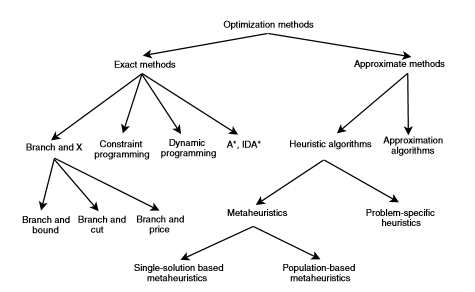
\includegraphics[width=0.8\textwidth]{mem/images/meta.png}
\caption{Optimisation methods}
\end{figure}

On the one hand, \textit{exacts methods} are those which ensure that, if there is an optimal solution to the facing problem they will be able to find it. However, these methods that guarantees reaching the optimal solution, they have a important drawback, its performance. Assuring the optimal solution implies increasing the computational work and hence more time to obtain the solution.

On the other hand, \textit{approximated methods} are very popular nowadays even though they do not guarantee reaching the optimal solution for a problem. Nevertheless, approximated methods can obtain high quality solutions in an assumable time due they set a balance between computational performance and solution quality. 

Approximated methods can be divided in two categories: \textit{heuristic algorithms} and \textit{metaheuristics algorithms}. However, this work it is focus primarily in \textit{metaheuristics algorithm} and even more specifically in the field of \textit{evolutionary algorithms}.

Evolutionary algorithms~(EA) develop the metaphor of natural evolution, the survival of the fittest individual\cite{eiben}. This is, given a population of individuals in some environment with limited resources, the competition for surviving causes natural selection and the fittest individuals are more likely to survive and reproduce. Nevertheless, there are several variants of EA and they can be classified as:
\begin{enumerate}
    \item Genetic Algorithms\cite{Whitley1994, Algorithms2004, Sivanandam2008}.
    \item Evolutionary Strategies\cite{Beyer2002, Hansen2017}.
    \item Differential Evolution\cite{Algorithm2006, DE1, DE2, DE3}.
\end{enumerate}

Considering the field of optimisation problems, the natural evolution metaphor is develop as follows:
\begin{enumerate}
    \item The problem to solve and its bounds is the environment with limited resources.
    \item A set of random initial solutions for the given problem are the first individuals at generation zero. 
    \item The population of individuals reproduce between each other applying genetic operators to generate offspring. Commonly combination and mutation.
    \item At each generation, the individuals within a population compete and the fittest individuals (the better quality solutions) survive.
    \item Steps three and four are repeated until reaching the stop condition.
\end{enumerate}
Generally, the before metaphor can be shown as a pseudo-code\cite{eiben}:

\begin{algorithm}[!h]
  INITIALISE population with random candidate solutions\;
  EVALUATE each candidate\;
  \While{not StopCriteria satisfied}{
    SELECT parents\;
    RECOMBINE pairs of parents\;
    MUTATE the result offspring\;
    EVALUATE new candidates\;
    SELECT individuals for the next generation\; 
  }
  \caption{General scheme of an EA.}
\end{algorithm}

%%%%%%%%%%%%%%%%%%%%%%%%%%%%%%%%%%%%%%%%%%%%%%%%%%%%%%%%%%%%%%%%%%%%%%%%%%%%%%%%%%%%%%%
\newpage
\section{Menu Planning Problem}

The Menu Planning Problem \textit{(MPP)} is a well-known NP-Problem which has been trying to computerise since 1960\cite{Ngo2016}. In essence, the MPP is to find a set of dishes combination which satisfies some restrictions of budge, variety and nutritional requirements for a \textit{n} days sequence. In addition, it can include other constraints such as user preferences, cooking time or the number for meals each day.
Traditionally, the MPP's main objective is to minimise the total cost of the meals for each day\cite{Ngo2016, Moreira2018} but it also supports other objective functions like maximising the variability or minimising the cooking time.

Furthermore, the MPP can be studied as a multi-objective problem\cite{Seljak2009, Moreira2018} if the amounts of nutrients requirements and cost of the meals are considered independent objectives. This approach leads to reduce the MPP to a Multi-dimensional Knapsack Problem \textit{(MDKP)} where the maximum amount of each nutrient define the limit of the multiple dimensions. However, the MPP is also studying as a single-objective problem where mainly research define the objective function as the total cost of the meals. For instance, a single-objective approach for the MPP is in\cite{Moreira2018} where the authors proposed an evolutionary approach to solving the 5-day Single-Objective Menu Planning Problem composed by three meals daily, using as a function to minimise the total cost of the designed menus. In addition, the set of constraints that the researchers defined to this problem are moderately different from the usual constraints set for the typical MPP. In this occasion, the authors set the student age group, the school category, school duration time, school location, variety of preparations, the maximum amount to be paid for each meal and finally, the lower and upper limits of macro-nutrients as the constraints set to be satisfied for each solution to be considered feasible. Within this research, the authors used the generic Genetic Algorithm (GA) for the computational experiments. The results obtained from the generic GA where compared with a Greedy-based approach. The results prove that the GA outperforms the Greedy-based approach when the limit values of the meals are fixed at R\$ 2.00 for breakfast, R\$ 4.00 for lunch and R\$ 2.00 for the snack. (BRL - R\$ 1.0 ~~ USD - \$ 0.31).

In the other hand, in the paper\cite{Funabiki2011}, the authors refer to the Two-phase Cooking N-day Menu Planning Problem where the objective is to maximise the preferences among the selected foods in the menu plan. The conditions which shape the set of constraints that must be satisfied are only three. The total cooking time of any day must not exceed the limit specified, only foods that which allow two-phase cooking can be selected for two-phase cooking and finally, the food cannot be repeated more times than a certain repeat constraint. In order to face this problem, the researchers used a simple greedy method prioritising the user-specified preference with the cooking time of each food.

Eventually, another study where the MPP is faced as a single-objective problem is\cite{Sufahani2014}. Here, the authors set up a mathematical model to solve the MPP considering only one objective function. The model's goal is to minimise the budget provided by the government subject to the restriction of trying to maximise the variety of dishes. Furthermore, the model tries to create menus in such a way they maximise the nutritional requirements. For the computational experiments, the researchers programmed an Integer Programming algorithm in Matlab using LPSolve. Furthermore, the given results, taking into account that the optimal solution was found within one second, are better compared to other heuristics like GA.

As can be seen, there is a certain variety whitin the optimisation methods for solving the single-objective MPP approach. Despite that, Evolutionary Computing \textit{(EC)} techniques, such as GA, are mostly cited in the related bibliography as a good choice\cite{Ngo2016, Seljak2009, Moreira2018}. 

Nevertheless, there is not any study which compares the performance and results between the multi-objective MPP and the single-objective MPP. 
\newpage{\pagestyle{empty}}
\chapter{Algorithms}\label{ref:algorithm}
\section{Multiobjective Evolutionary Algorithm Based on Decomposition}
Multiobjective Evolutionary Algorithm Based on Decomposition (MOEA/D) is an evolutionary algorithm for multiobjective optimisation proposed by Qingfu Zhang and Hui Li in 2007\cite{Zhang2007}. The underlying idea behind this algorithm is to decompose a multiobjective optimisation problem into a number of scalar optimisation sub-problems and optimises them simultaneously. It also harnesses in the well-known feature of Pareto optimal solutions to a MOP, which sustains that an optimal solution for a scalar optimisation problem with an objective function as the aggregation of all the $f_{i}$ could be the same as the Pareto optimal solution for the MOP\cite{Zhang2007}.

The decomposition approach of MOEA/D takes place where the algorithm decomposes a MOP into \textit{N} sub-problems and simultaneously optimises every single sub-problem at each generation. Furthermore it establish some relations between sub-problems and organised them in neighbourhoods. These neighbourhoods are shaped by sub-problems which coefficient vectors are very similar to each other and every single sub-problem is optimised based on its neighbouring sub-problems information. Therefore, the optimal solution for two neighbouring sub-problems should be very similar\cite{Zhang2007}.

On the other hand, the process of decompose a MOP into \textit{N} sub-problems can be done from some different approaches. However, as the authors referred\cite{Zhang2007} it this paper the MOEA/D uses the Tchebycheff Approach\cite{Ma2018} to decompose a MOP. Formally, the Tchebycheff Approach it is defined as follows:
\[
min\quad g^{te}(x|\lambda,z^{*}) = max_{i=1}^{m}\{\lambda_{i}|f_{i}(x)-z_{i}^{*}|\}
\]

where $z^{*} = (z^{*}_{1}, ..., z^{*}_{m})$ is the reference point with the best solution founds so far for each sub-problem and $\lambda_{i} = (\lambda_{i,1}, ..., \lambda_{i,m})$ is a even spread weight vector for each sub-problem \textit{i}.

In addition, MOEA/D version implemented in this paper works as follows. It takes a MOP, the population size, a stopping criterion and the number of neighbours for each neighbourhood. The number of sub-problems in this implementation are the MOP's objectives. Then, it starts by randomly generate \textit{N} even spread weight vectors and compute the Euclidean distance between each others to shape the neighbourhoods, generates an initial random population and computes the reference point $Z^{*}$. After the initialisation phase, it goes into the main loop where, until the stopping criteria is not satisfied, the algorithm preforms theses steps for each individual of the population:
\begin{itemize}
  \item Reproduction: generates a new child individual from two randomly selected neighbours \textit{l, k}.
  \item Improve: maintains the new child under the limits of the problem's search space.
  \item UpdateZ: updates the reference point by comparing it with each new child individual.
  \item Update Neighbours: if the new child individual performs better than any neighbours, replaces the neighbour with the brand new individual.
\end{itemize}
Finally, MOEA/D returns the PF's points found. \\

Concretely, the algorithm can be outlined as follows: \\

\begin{algorithm}[H]
  \KwData{MOP, PopSize, StopCriteria, Neighbours}
  \KwResult{PF}
  SetRandomWeightVectors()\;
  EuclideanDistance()\;
  GenerateRandomPopulation()\;
  InitializeZ()\;
  \While{not StopCriteria satisfied}{
    \For{each sub-problem do} {
      l,k = getRandomNeigbours()\;
      child = reproduce(l, k)\;
      child = improve(child)\;
      updateZ(child)\;
      updateNeighbouringSolutions(child)\;
    }
  }
  \caption{MOEA/D version of this thesis.}
\end{algorithm}
\section{Strength Pareto Evolutionary Algorithm}
\section{Non-dominated Sorting Genetic Algorithm II}


\newpage{\pagestyle{empty}}
\chapter{Experimental Evaluation}\label{ref:results}
%%%%%%%%%%%%%%%%%%%%%%%%%%%%%%%%%%%%%%%%%%%%%%%%%%%%%%

In this chapter, the experimental evaluation of MOEA/D will be introduced. %In order to achieve an accurate comparison of MOEA/D with the results obtained in \cite{Miranda2018} by other algorithms mentioned before (NSGA-II and SPEA-2),%
The algorithm and the experimental evaluation were developed through the same framework called Metaheuristic-based Extensible Tool for Cooperative Optimisation (METCO)~\footnote{Available at: https://github.com/PAL-ULL/software-metco} proposed in \cite{METCO}.
In addition, the experiment were executed on a Debian GNU/Linux computer with four AMD Opteron processors at 2.8GHz and 64 GB RAM. Each run was repeated 25 times considering 1e8 evaluations as the stop criteria.

Furthermore, with the aim of statistically supporting the conclusions extracted, the following the evaluation procedure was applied. The \textit{hypervolume~(HV)}~\cite{HYPER} was the metric selected to compare the different configurations of MOEA/D and the \textit{Shapiro-Wilk, Levene, ANOVA or Welch} test were considered for results which follow a normal distribution or \textit{Kruskal-Wallis} test otherwise. 
%%%%%%%%%%%%%%%%%%%%%%%%%%%%%%%%%%%%%%%%%%%%%%%%%%%%%%%%
\section{Instances}
For this evaluation, a total number of 67 different courses were available group together in three different files:
\begin{itemize}
    \item $l_{st}$: 19 starters.
    \item $l_{mc}$: 34 main courses.
    \item $l_{ds}$: 14 desserts.
\end{itemize}
Besides, the structure of every file is an CSV file with the following fields:
\begin{itemize}
    \item Name of the course.
    \item Price of the course.
    \item Binary list of different allergens in case whether the course contains or not the allergen.
    \item Incompatibilities.
    \item Amount of the different nutrients.
    \item Food groups which belongs the course.
\end{itemize}
%%%%%%%%%%%%%%%%%%%%%%%%%%%%%%%%%%%%%%%%%%%%%%%
\section{Parameter Setting}
In this preliminary experiment, the main goal was to find which values of the MOEA/D\cite{Zhang2007} parameters provide the best configuration facing the MPP formulation considered in this Master Thesis. The list of MOEA/D parameters is:
\begin{itemize}
    \item Population size.
    \item Neighbourhood size.
    \item Mutation probability that was set at 0.05.
    \item Crossover probability which was set at 1.
\end{itemize}
At this point, it is worth mentioning that MPP takes one parameter which defines the number of different days, for which the menu plan will be designed, that in this preliminary experiment was set to \textbf{20 days}. 
The comments of the authors of MOEA/D algorithm in \cite{Zhang2007} about the performance of the algorithm with very small or large neighbourhood sizes and the effect of the population size on its performance were took into account when designing this experiment. Bearing the above in mind, a wide range of values were considered. Particularly, five different values for the population size and neighbourhood size were set in order to obtain 25 different configurations of MOEA/D. The values are:
\begin{itemize}
    \item Population size: 25, 80, 140, 190, 250.
    \item Neighbourhood size: 0.4, 0.3, 0.25, 0.2, 0.16 percentage of the total population size.
\end{itemize}
Table \ref{ranking} shows the ranking of all MOEA/D configuration for a 20-days MPP related to the hypervolume values obtained at the end of the executions. The ranking \textit{(R)} was calculated considering the number of times that one configuration statistically outperforms other configurations \textit{(W)} and the number of times that it was outperformed by other configurations \textit{(L)}: 
\[ 
R = W - L
\]
Configuration A statistically outperforms configuration B if the p-value, obtained after performing a pairwise comparison of both approaches by following the statistical testing procedure described at the beginning of this chapter, is lower than the significance level $\alpha = 0.05$ , and if at the same time, A provides a higher mean and median of the hypervolume at the end of the runs.

Even though there is not a significant control of the best ranked configuration in Table \ref{ranking} with only 9 wins over 24 other configurations, the MOEA/D configuration with a population size of 140 individuals and 42 individuals per neighbourhood seems to be the best one. Thus, this is the configuration chosen for the next experiment.
% Please add the following required packages to your document preamble:
% \usepackage{graphicx}
\begin{table}[!h]
\centering
\resizebox{1.05\textwidth}{!}{%
\begin{tabular}{|c|c|c|c|c|c|c|c|c|c|}
\hline
\textbf{Configuration}            & \textbf{Min.} & \textbf{1st Qu.} & \textbf{Median} & \textbf{Mean} & \textbf{3rd Qu.} & \textbf{Max.} & \textbf{W} & \textbf{L} & \textbf{Ranking} \\ \hline
MOEA\_D\_PopSize\_140\_Neihb\_42  & 0.7161        & 0.7733           & 0.7839          & 0.7834        & 0.8087           & 0.8435        & 9          & 0          & 9                \\ \hline
MOEA\_D\_PopSize\_250\_Neihb\_50  & 0.7270        & 0.7635           & 0.7737          & 0.7775        & 0.7930           & 0.8213        & 2          & 0          & 2                \\ \hline
MOEA\_D\_PopSize\_80\_Neihb\_16   & 0.7306        & 0.7655           & 0.7787          & 0.7774        & 0.7945           & 0.8342        & 2          & 0          & 2                \\ \hline
MOEA\_D\_PopSize\_140\_Neihb\_35  & 0.7388        & 0.7583           & 0.7671          & 0.7728        & 0.7914           & 0.8188        & 1          & 0          & 1                \\ \hline
MOEA\_D\_PopSize\_190\_Neihb\_48  & 0.7216        & 0.7521           & 0.7670          & 0.7688        & 0.7842           & 0.8034        & 0          & 0          & 0                \\ \hline
MOEA\_D\_PopSize\_25\_Neihb\_10   & 0.7228        & 0.7563           & 0.7669          & 0.7686        & 0.7805           & 0.8250        & 0          & 0          & 0                \\ \hline
MOEA\_D\_PopSize\_25\_Neihb\_4    & 0.7363        & 0.7490           & 0.7628          & 0.7682        & 0.7817           & 0.8174        & 0          & 0          & 0                \\ \hline
MOEA\_D\_PopSize\_80\_Neihb\_13   & 0.7231        & 0.7563           & 0.7690          & 0.7691        & 0.7874           & 0.8143        & 0          & 0          & 0                \\ \hline
MOEA\_D\_PopSize\_25\_Neihb\_8    & 0.7384        & 0.7490           & 0.7725          & 0.7716        & 0.7884           & 0.7989        & 0          & 0          & 0                \\ \hline
MOEA\_D\_PopSize\_140\_Neihb\_28  & 0.7299        & 0.7583           & 0.7715          & 0.7715        & 0.7892           & 0.8005        & 0          & 0          & 0                \\ \hline
MOEA\_D\_PopSize\_80\_Neihb\_32   & 0.7256        & 0.7428           & 0.7708          & 0.7675        & 0.7840           & 0.8190        & 0          & 0          & 0                \\ \hline
MOEA\_D\_PopSize\_250\_Neihb\_62  & 0.7244        & 0.7577           & 0.7733          & 0.7702        & 0.7847           & 0.8189        & 0          & 0          & 0                \\ \hline
MOEA\_D\_PopSize\_80\_Neihb\_24   & 0.7234        & 0.7540           & 0.7710          & 0.7712        & 0.7843           & 0.8158        & 0          & 0          & 0                \\ \hline
MOEA\_D\_PopSize\_140\_Neihb\_22  & 0.7292        & 0.7504           & 0.7728          & 0.7684        & 0.7813           & 0.8231        & 0          & 0          & 0                \\ \hline
MOEA\_D\_PopSize\_250\_Neihb\_100 & 0.7328        & 0.7501           & 0.7775          & 0.7721        & 0.7925           & 0.8253        & 0          & 0          & 0                \\ \hline
MOEA\_D\_PopSize\_25\_Neihb\_6    & 0.7211        & 0.7506           & 0.7673          & 0.7706        & 0.7897           & 0.8300        & 0          & 0          & 0                \\ \hline
MOEA\_D\_PopSize\_250\_Neihb\_40  & 0.7158        & 0.7507           & 0.7737          & 0.7674        & 0.7811           & 0.8155        & 0          & 1          & -1               \\ \hline
MOEA\_D\_PopSize\_190\_Neihb\_57  & 0.6755        & 0.7441           & 0.7698          & 0.7655        & 0.7809           & 0.8135        & 0          & 1          & -1               \\ \hline
MOEA\_D\_PopSize\_140\_Neihb\_56  & 0.7149        & 0.7472           & 0.7704          & 0.7664        & 0.7799           & 0.8311        & 0          & 1          & -1               \\ \hline
MOEA\_D\_PopSize\_250\_Neihb\_75  & 0.7078        & 0.7443           & 0.7664          & 0.7637        & 0.7765           & 0.8143        & 0          & 1          & -1               \\ \hline
MOEA\_D\_PopSize\_190\_Neihb\_76  & 0.7374        & 0.7546           & 0.7694          & 0.7685        & 0.7818           & 0.8018        & 0          & 1          & -1               \\ \hline
MOEA\_D\_PopSize\_25\_Neihb\_5    & 0.7299        & 0.7494           & 0.7683          & 0.7672        & 0.7802           & 0.8180        & 0          & 1          & -1               \\ \hline
MOEA\_D\_PopSize\_80\_Neihb\_20   & 0.7269        & 0.7484           & 0.7676          & 0.7663        & 0.7732           & 0.8217        & 0          & 1          & -1               \\ \hline
MOEA\_D\_PopSize\_190\_Neihb\_38  & 0.7224        & 0.7515           & 0.7643          & 0.7634        & 0.7780           & 0.8113        & 0          & 3          & -3               \\ \hline
MOEA\_D\_PopSize\_190\_Neihb\_30  & 0.7280        & 0.7494           & 0.7581          & 0.7607        & 0.7698           & 0.7978        & 0          & 4          & -4               \\ \hline
\end{tabular}%
}
\caption{Ranking of all MOEA/D configurations}
\label{ranking}
\end{table}

\newpage

\section{Problem size variation}
In this experiment, the main goal was to analyse how the problem dimension affects in the performance of the best MOEA/D configuration found so far for MPP. For that reason, other 25 independent executions of MOEA/D with 140 individuals in the population and neighbourhoods of 42 individuals were run for instances of the MPP of 5, 10 and 40 days MPP. Table \ref{table:MOEA_5_10} below shows the minimum, median, mean and maximum hypervolume values obtained. The best MOEA/D configuration is compared to the best results for NSGA-II and SPEA-2 for every different MPP instance. As it can be observed, both NSGA-II and SPEA-2 outperformed MOEA/D in every different MPP instance with statistically significant differences.


% Please add the following required packages to your document preamble:
% \usepackage{graphicx}
\begin{table}[H]
\centering
\resizebox{\textwidth}{!}{%
\begin{tabular}{|c|c|c|c|c|}
\hline
\textbf{Algorithm} & \textbf{Min} & \textbf{Median} & \textbf{Mean} & \textbf{Max} \\ \hline
MOEA\_D\_PopSize\_140\_Neihb\_42\_days\_5 & 0.747678 & 0.827983 & 0.827358 & 0.873078 \\ \hline
MOEA\_D\_PopSize\_140\_Neihb\_42\_days\_10 & 0.743725 & 0.78073 & 0.78353884 & 0.83404 \\ \hline
\end{tabular}%
}
\caption{Results of MOEA/D with different MPP sizes.}
\label{table:MOEA_5_10}
\end{table}


%Moreover, comparing the results of the previous work done with this novel MPP formulation in\cite{Miranda2018}, even though the authors set the number of evaluations at 4e8 the average hypervolume value at 1e8 evaluations for, i.e 10-days MPP instances can be seen in the following Table \ref{table:compare}. The results shows how every chosen configuration of~NSGA-II and SPEA-2 outperforms the best configuration found so far for MOEA/D facing 10-days MPP. 
%
%\begin{table}[!ht]
\centering
\begin{tabular}{|c|c|}
\hline
\textbf{Algorithm} & \textbf{Mean HV at 1e8} \\ \hline
MOEA\_D\_PopSize\_140\_Neihb\_42 & 0.78353884 \\ \hline
NSGA2\_PopSize\_250\_pm\_0.1\_pc\_0.8 & \textbf{0.947955} \\ \hline
NSGA2\_PopSize\_250\_pm\_0.2\_pc\_0.8 & 0.9473880 \\ \hline
NSGA2\_PopSize\_250\_pm\_0.3\_pc\_0.8 & 0.9424957 \\ \hline
SPEA2\_PopSize\_100\_ArchSize\_100\_pm\_0.1\_pc\_0.8 & 0.9385228 \\ \hline
SPEA2\_PopSize\_100\_ArchSize\_100\_pm\_0.2\_pc\_0.8 & 0.9397660 \\ \hline
SPEA2\_PopSize\_100\_ArchSize\_100\_pm\_0.3\_pc\_0.8 & 0.9322837 \\ \hline
\end{tabular}
\caption{Comparison of the average HV values from different algorithms at 1e8ev.}
\label{table:compare}
\end{table}

Additionally, the Figure \ref{fig:previous_HV_5} shows how the average hypervolume value evolves and both NSGA-II and SPEA-2 reach considerably higher values than MOEA/D. With less than 0.2e8 evaluations, the average hypervolume value is noticeably higher than the average value reached by MOEA/D at 1e8 evaluations. The same comparison it is done in Figures \ref{fig:previous_HV_10}, \ref{fig:previous_HV_20} and\ref{fig:previous_HV_40} for 10, 20 and 40 days MPP instances, respectively.

\begin{figure}[H]
  \centering
  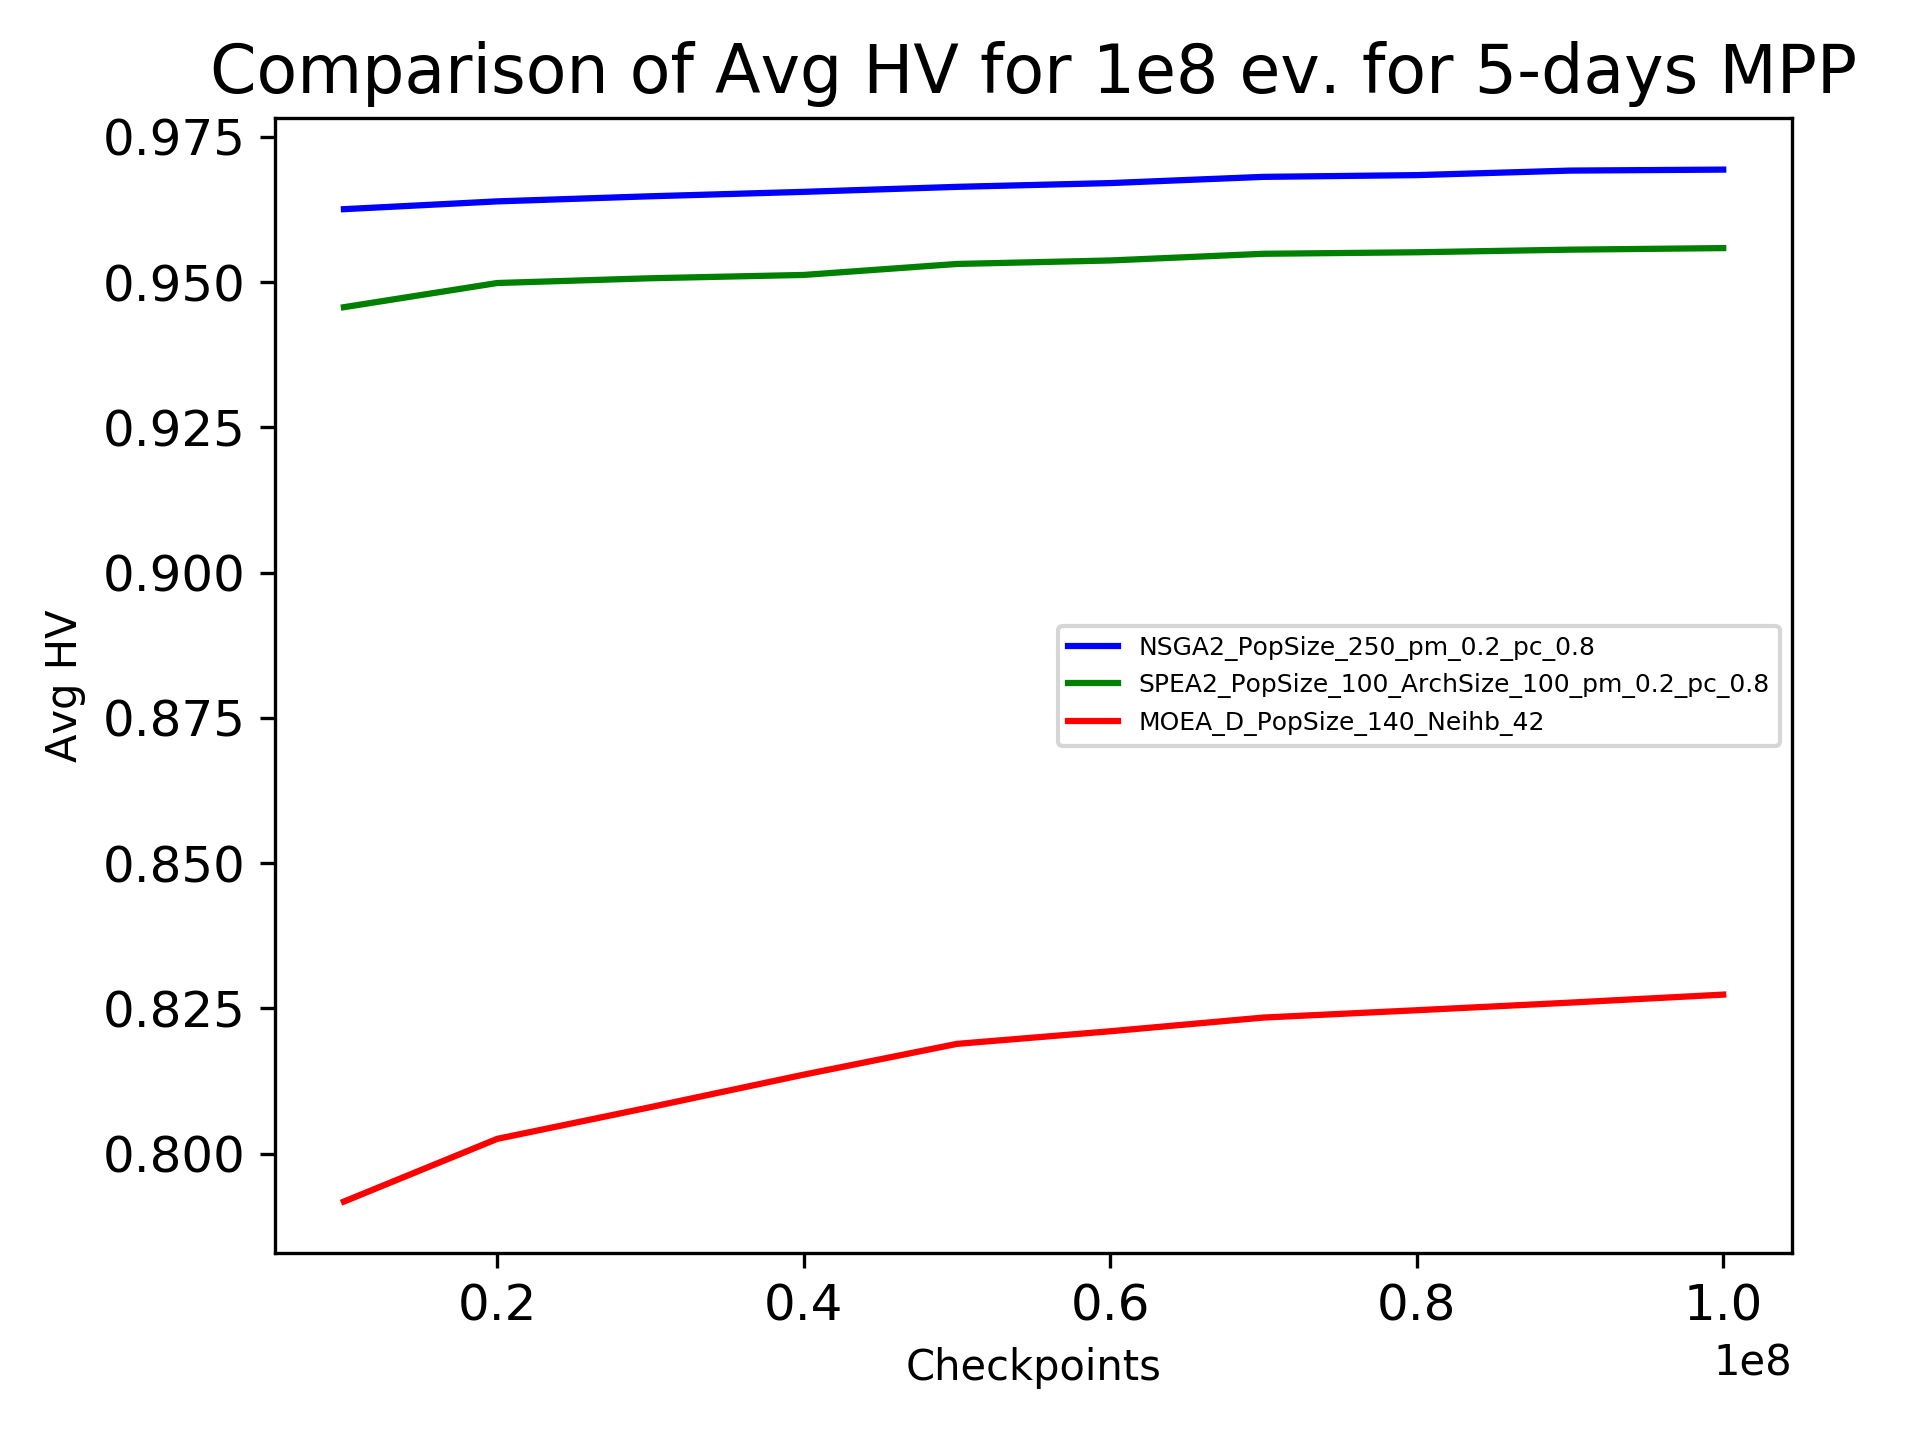
\includegraphics[width=1.0\linewidth]{../experiments/plots/avg_evolution_5_days.png}
\caption{Evolution of the average HV value for 5-days MPP at 1e8 evaluations.}
\label{fig:previous_HV_5}
\end{figure}

\begin{figure}[H]
  \centering
  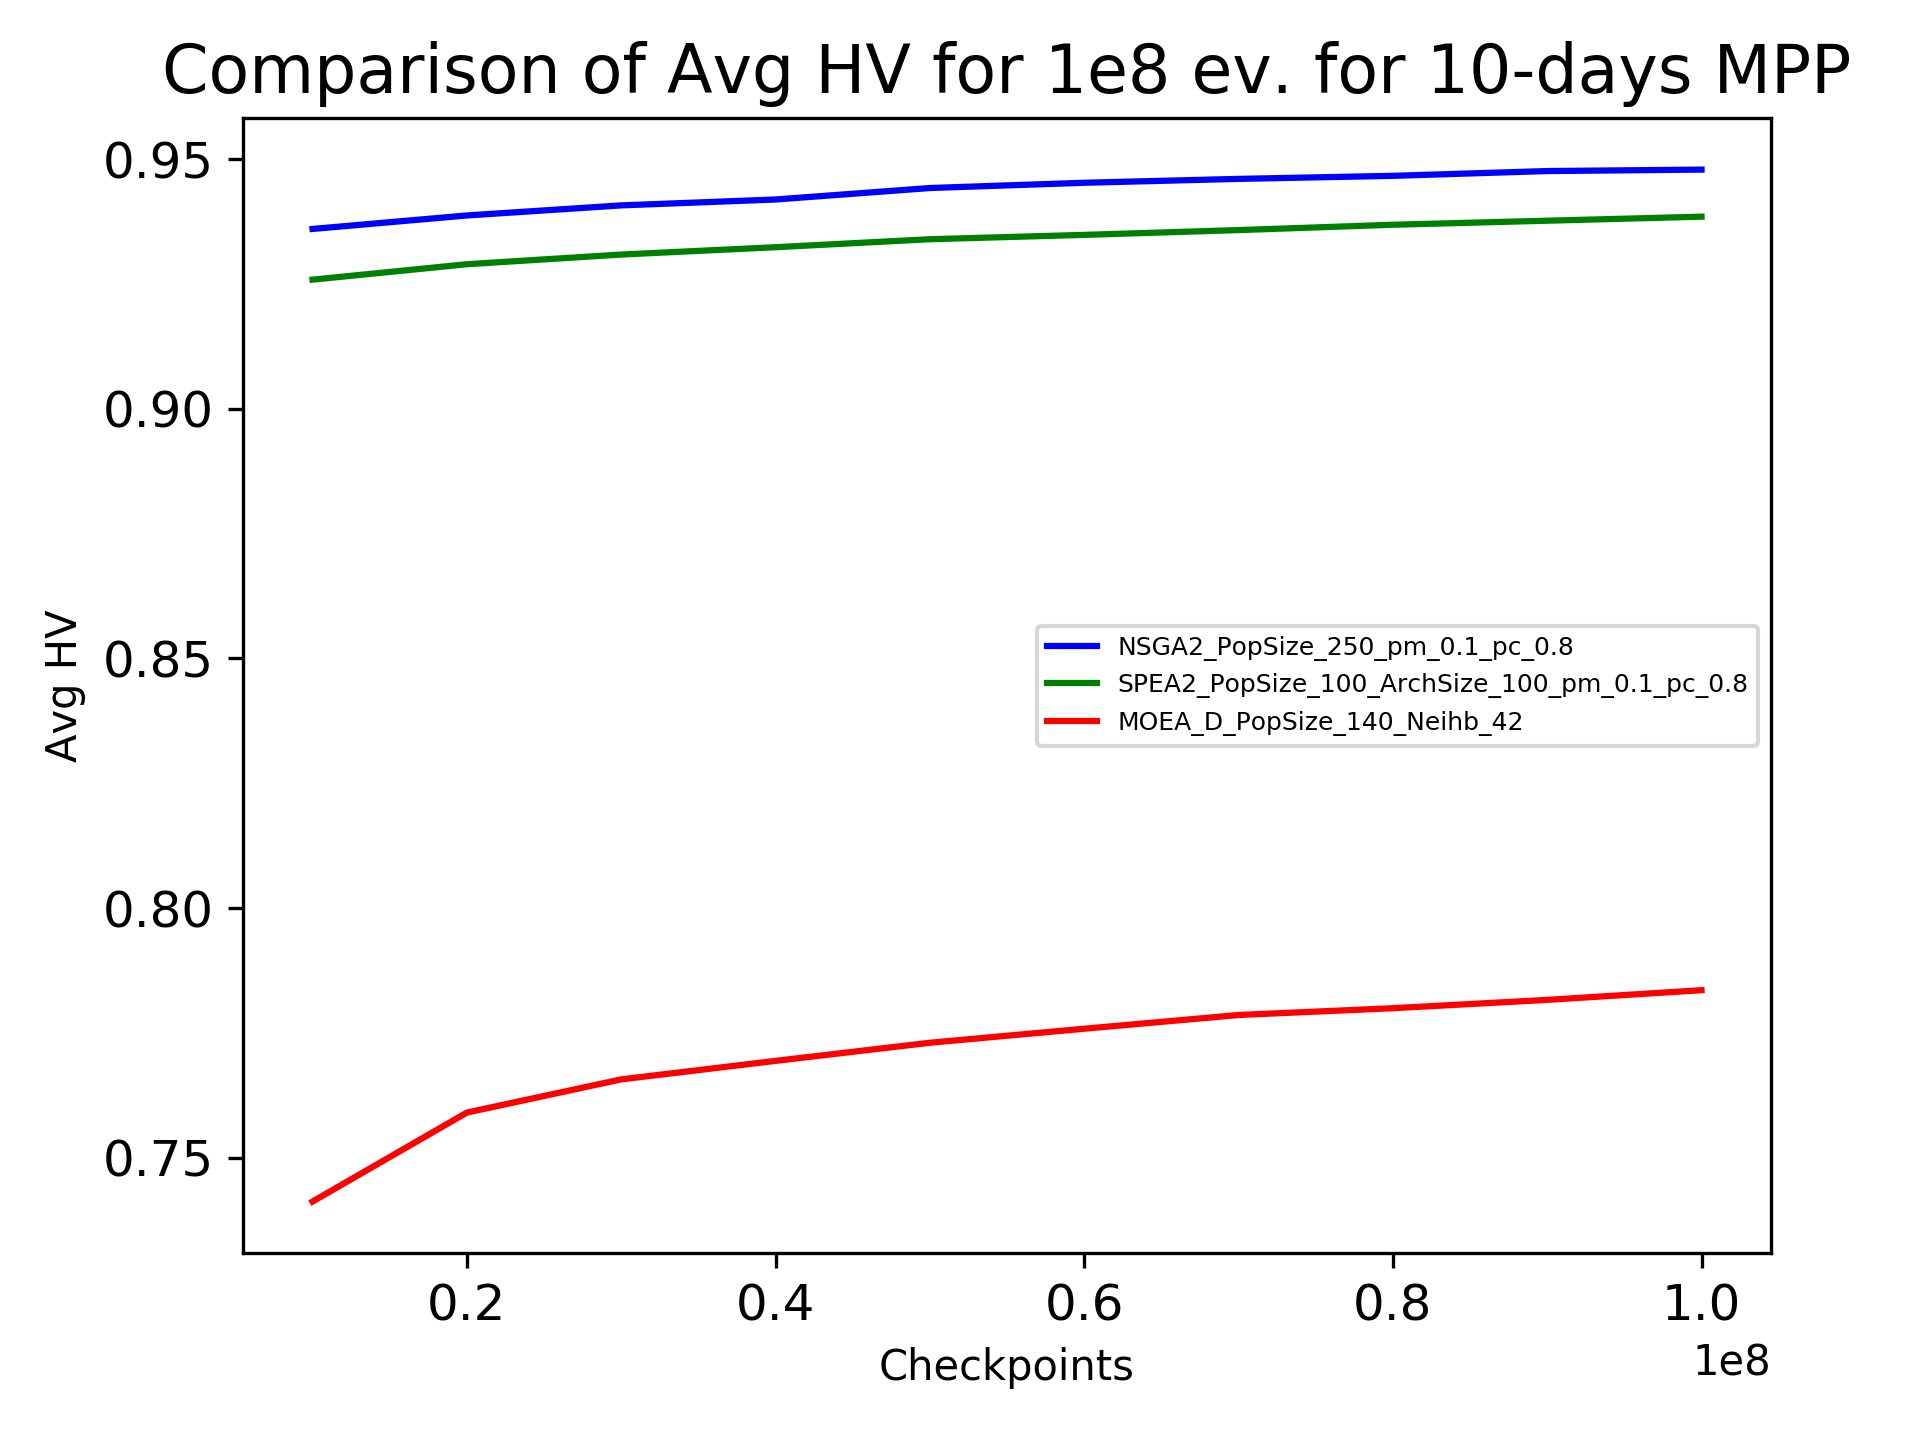
\includegraphics[width=1.0\linewidth]{../experiments/plots/avg_evolution_10_days.png}
\caption{Evolution of the average HV value for 10-days MPP at 1e8 evaluations.}
\label{fig:previous_HV_10}
\end{figure}

\begin{figure}[H]
  \centering
  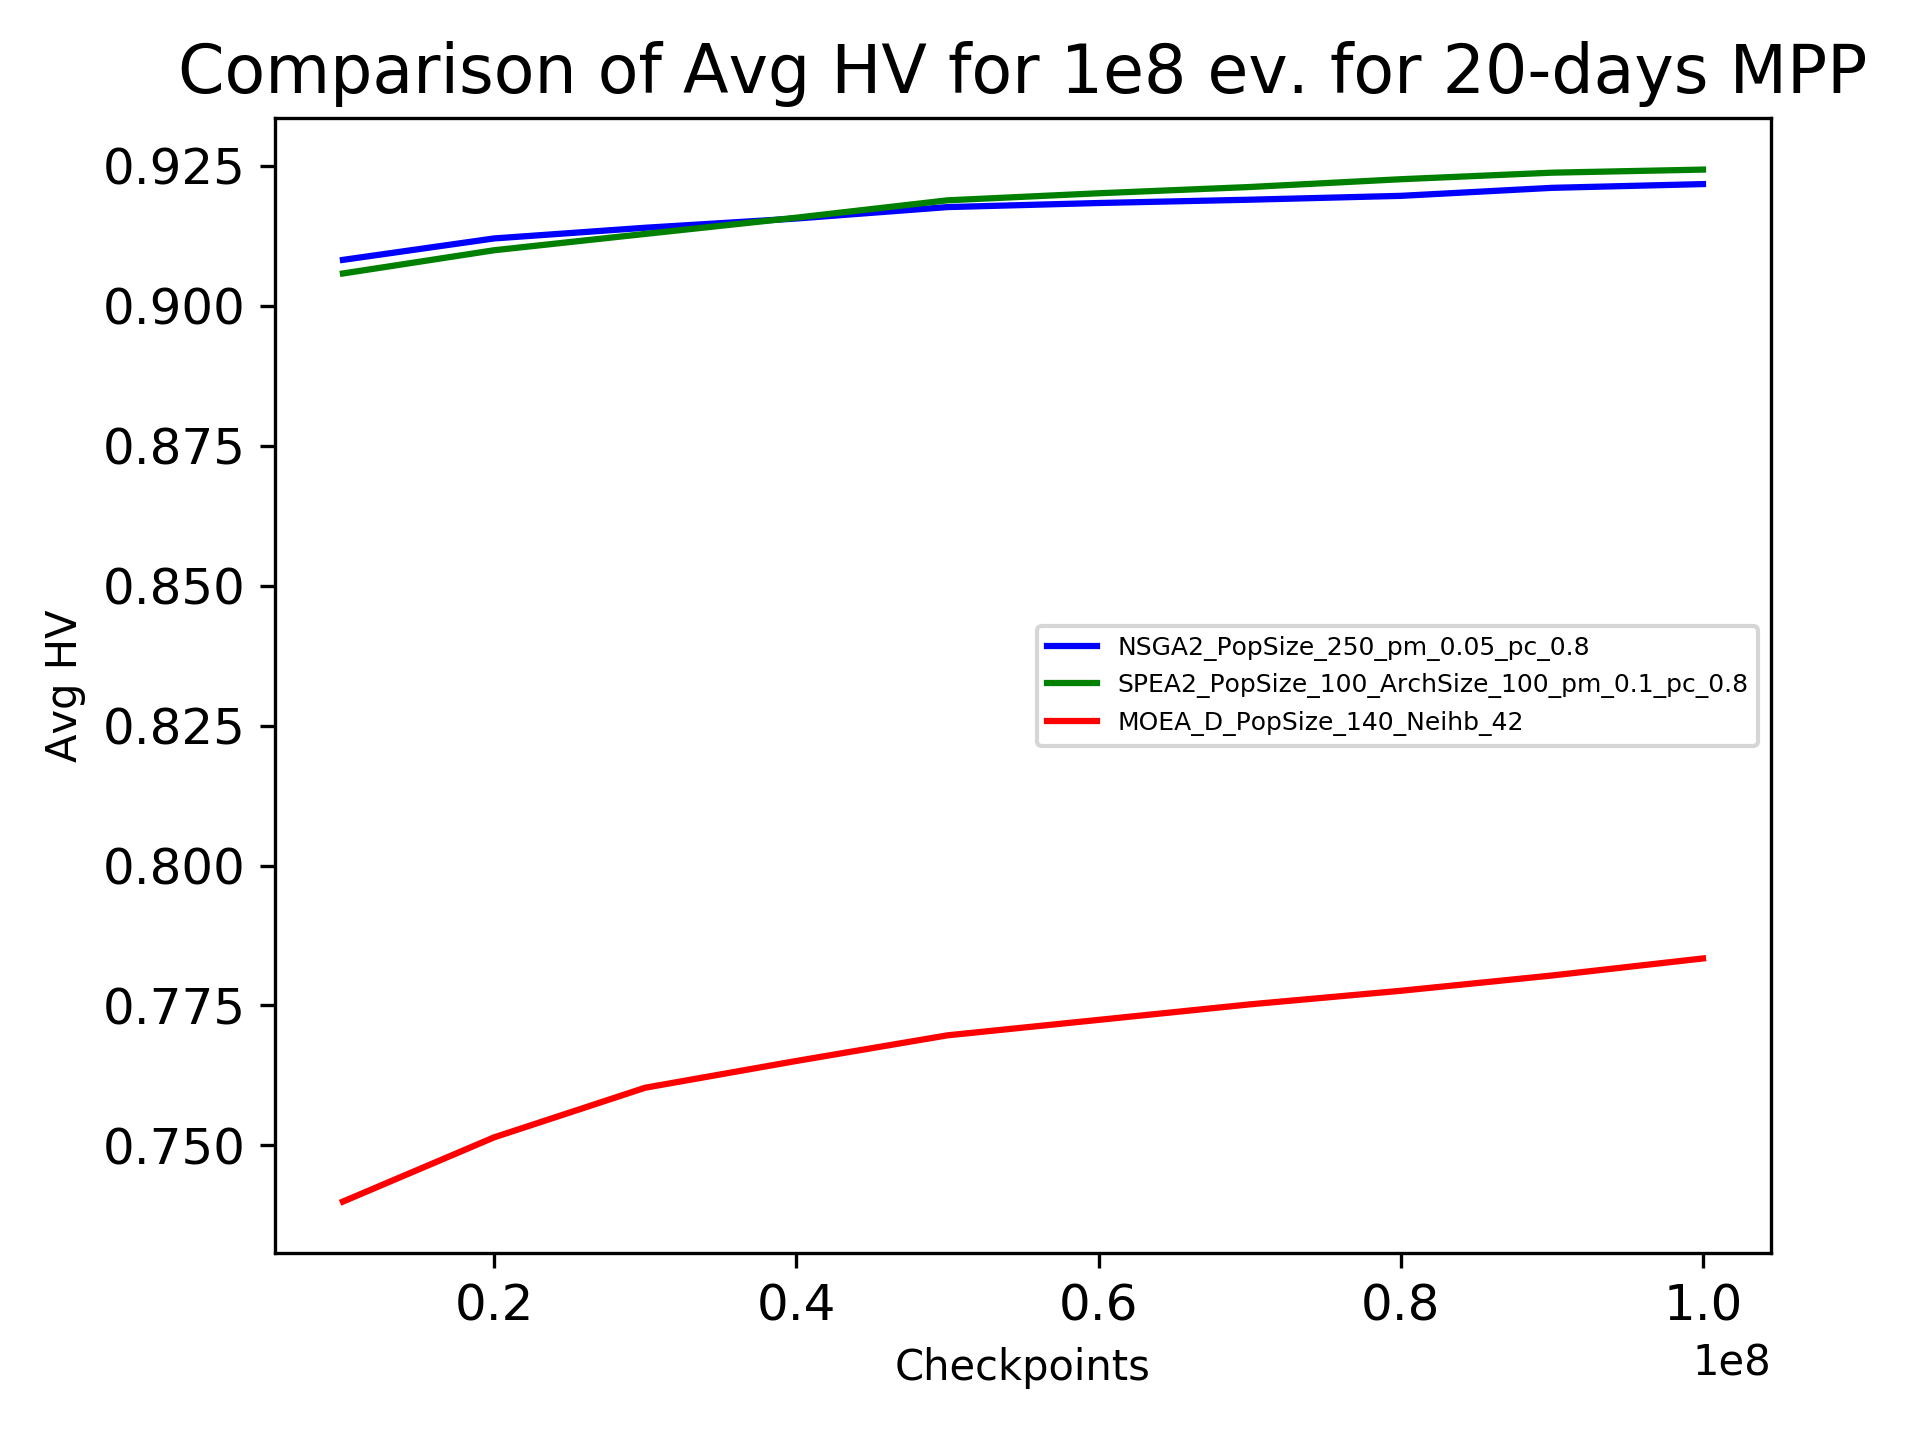
\includegraphics[width=1.0\linewidth]{../experiments/plots/avg_evolution_20_days.png}
\caption{Evolution of the average HV value for 20-days MPP at 1e8 evaluations.}
\label{fig:previous_HV_20}
\end{figure}

\begin{figure}[H]
  \centering
  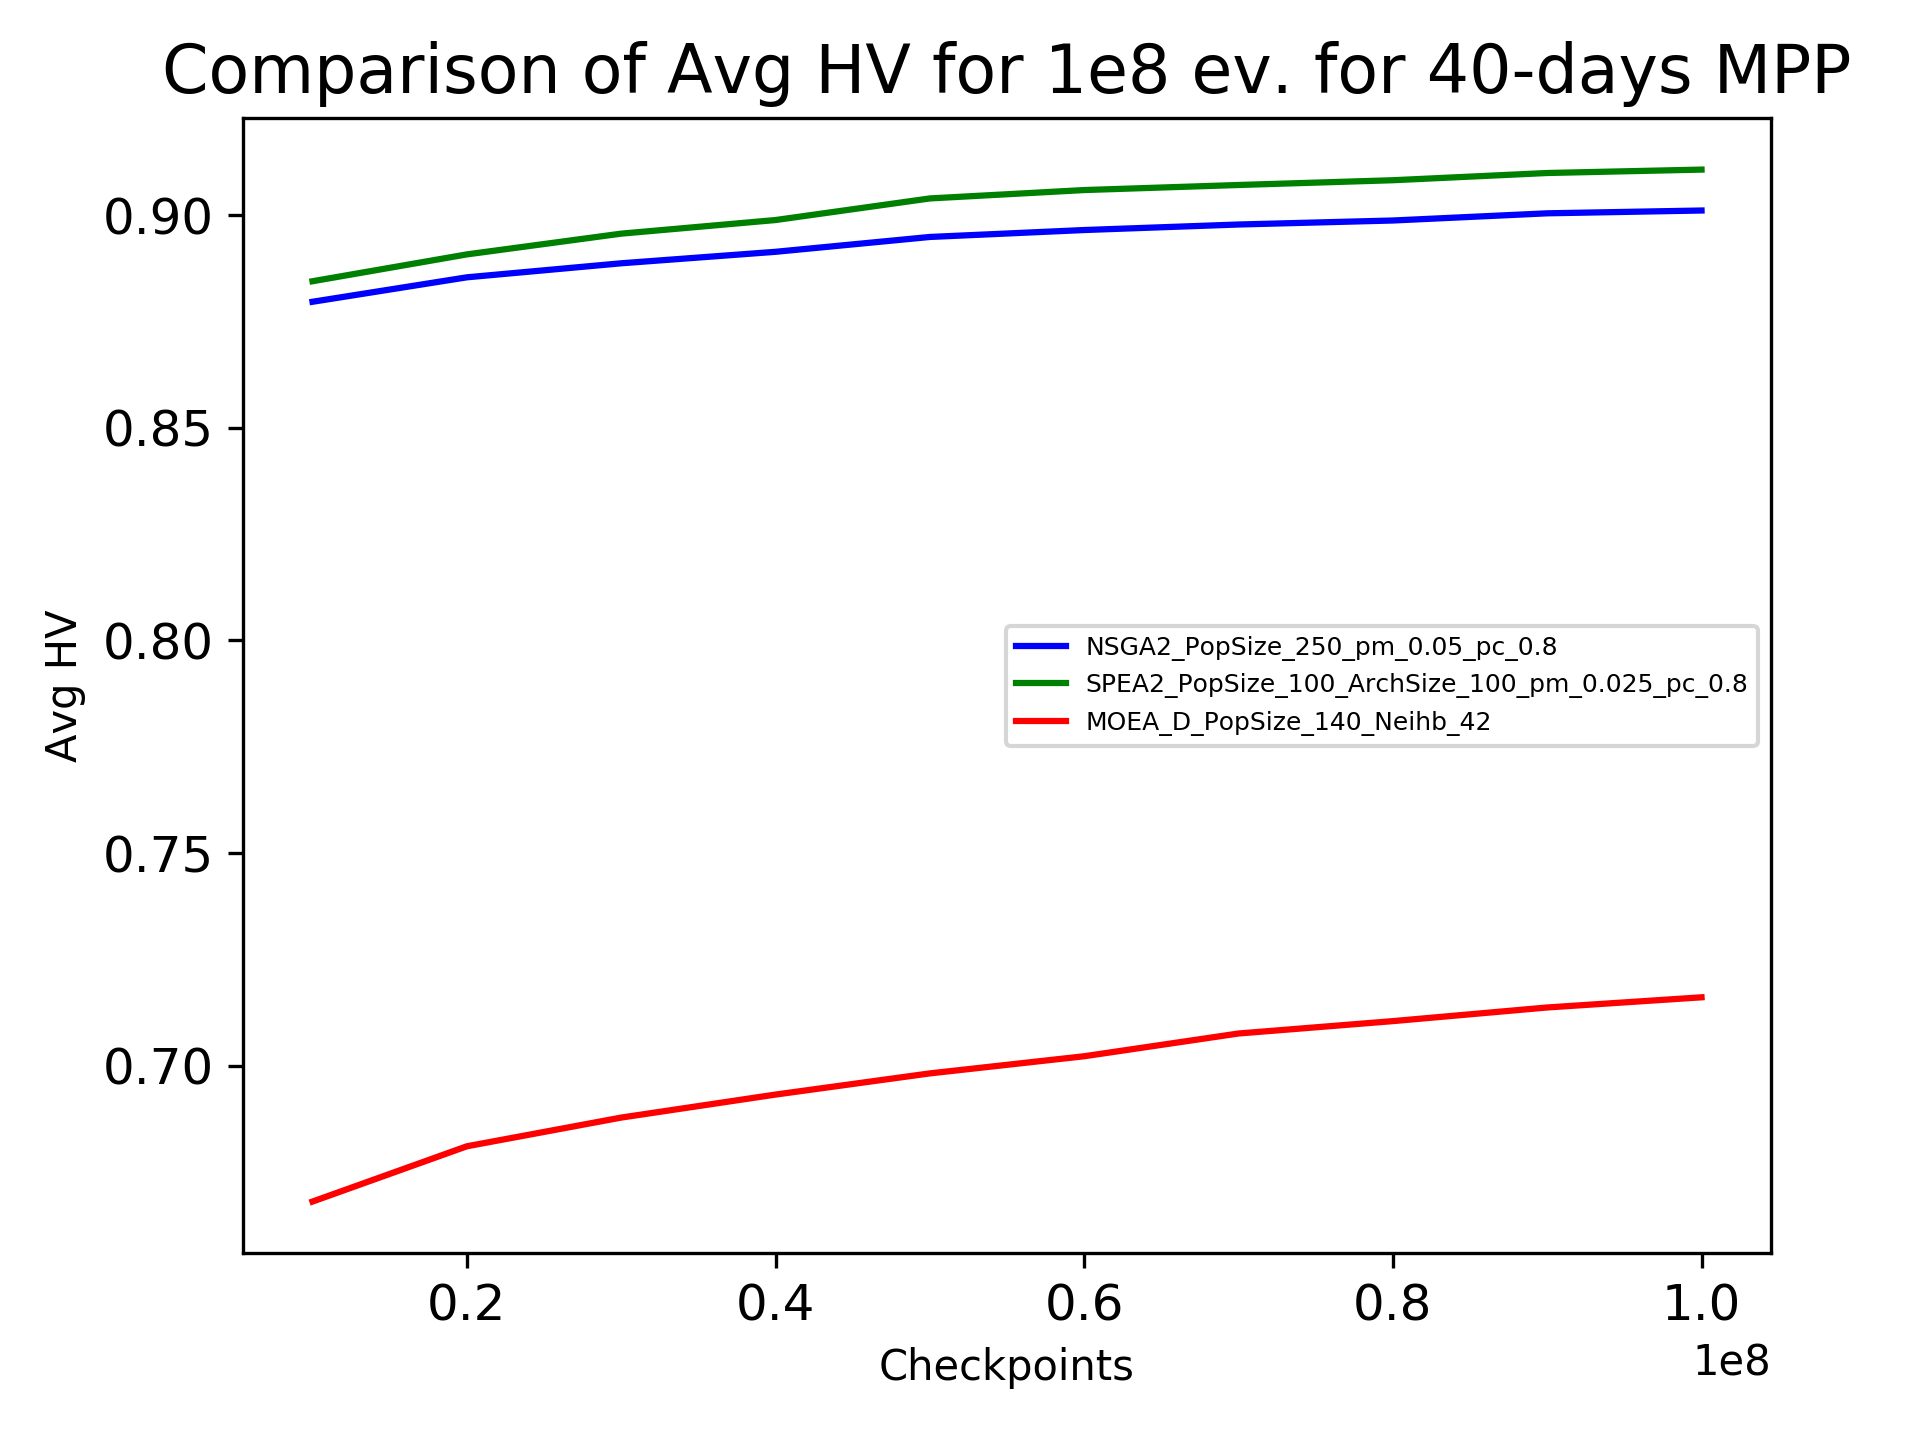
\includegraphics[width=1.0\linewidth]{../experiments/plots/avg_evolution_40_days.png}
\caption{Evolution of the average HV value for 40-days MPP at 1e8 evaluations.}
\label{fig:previous_HV_40}
\end{figure}


%%%%%%%%%%%%%%%%%%%%%%%%%%%%%%%%%%%%%%%%%%%%%%%%%%%%%%%%%%%%%%%%%%%%%
%Besides, Pareto Front representations of the final results from MOEA/D for every MPP instance after 1e8 evaluations are shown at Figures \ref{fig:front_comp_1}, \ref{fig:front_comp_2}, \ref{fig:front_comp_3} and \ref{fig:front_comp_4}. Although MOEA/D obtains menu plans with less degree of repetition, the total cost of the menu plan is slightly higher compared with the results obtained by NSGA-II and SPEA-2 with almost the same degree of repetition for 5-days, 10-days and 40-days MPP instances. These results are more than acceptable considering that MOEA/D performs four times less evaluations that NSGA-II and SPEA-2 in the experimental evaluation done in \cite{Miranda2018}.

\begin{figure}[H]
  \centering
  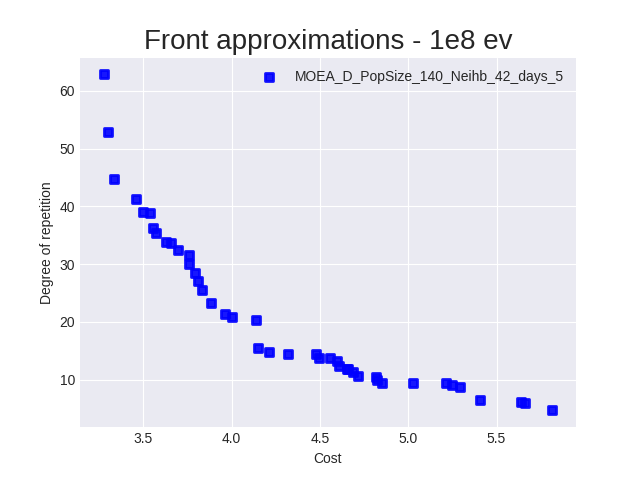
\includegraphics[width=1.0\linewidth]{../experiments/plots/fronts/5_days/MOEA_D_PopSize_140_Neihb_42_days_5_6.png}
\caption{Front approximation at 1e8 evaluations from best MOEA/D configuration found facing 5-days MPP.}
\label{fig:front_comp_1}
\end{figure}

\begin{figure}[H]
  \centering
  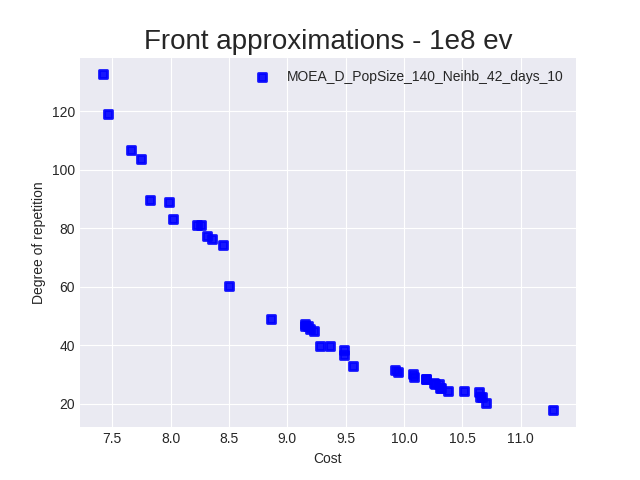
\includegraphics[width=1.0\linewidth]{../experiments/plots/fronts/10_days/MOEA_D_PopSize_140_Neihb_42_days_10_10.png}
\caption{Front approximation at 1e8 evaluations from best MOEA/D configuration found facing 10-days MPP.}
\label{fig:front_comp_2}
\end{figure}

\begin{figure}[H]
  \centering
  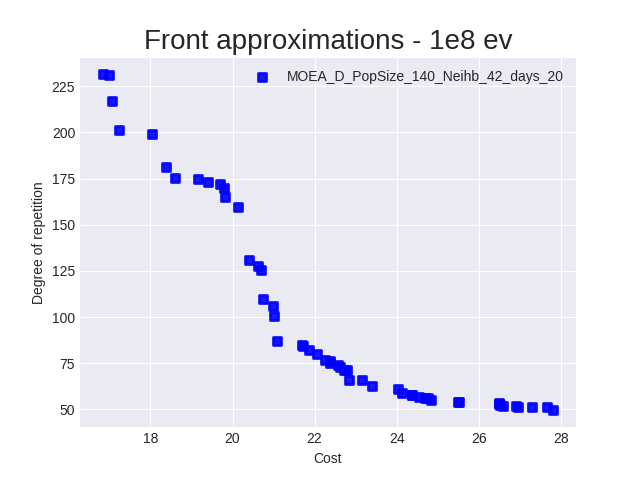
\includegraphics[width=1.0\linewidth]{../experiments/plots/fronts/20_days/MOEA_D_PopSize_140_Neihb_42_days_20_12.png}
\caption{Front approximation at 1e8 evaluations from best MOEA/D configuration found facing 20-days MPP.}
\label{fig:front_comp_3}
\end{figure}


\begin{figure}[H]
  \centering
  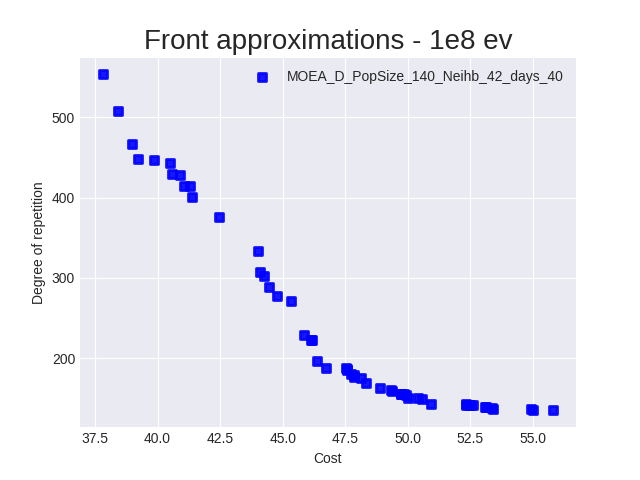
\includegraphics[width=1.0\linewidth]{../experiments/plots/fronts/40_days/MOEA_D_PopSize_140_Neihb_42_days_40_10.png}
\caption{Front approximation at 1e8 evaluations from best MOEA/D configuration found facing 40-days MPP.}
\label{fig:front_comp_4}
\end{figure}

%Lastly, due to the fact that the previous work and this experimental evaluation was done with the same framework and run in the same system, an reliable elapsed time comparison between the different algorithms can be made. The following Table \ref{table:time} shows the average time in hours for 25 independent runs for every compared algorithm. As results show, NSGA-II totally outperforms both SPEA-2 and MOEA/D for 5, 10, and 20-days MPP instances. However, surprisingly MOEA/D obtains quite faster but low quality results than NSGA-II and SPEA-2 for 40-days MPP.
% 
%% Please add the following required packages to your document preamble:
% \usepackage{graphicx}
\begin{table}[H]
\centering
\begin{tabular}{cc}
\hline
\multicolumn{1}{l}{\textbf{5-days MPP}} & \multicolumn{1}{l}{} \\ \hline
\multicolumn{1}{l}{Algorithm} & \multicolumn{1}{l}{Avg Elapsed Time (hours)} \\ \hline
NSGA-II & 5.579 \\
SPEA-2 & 7.734 \\
MOEA/D & 11.047 \\ \hline
\multicolumn{1}{l}{10-days MPP} & \multicolumn{1}{l}{} \\ \hline
\multicolumn{1}{l}{Algorithm} & \multicolumn{1}{l}{Avg Elapsed Time (hours)} \\ \hline
NSGA-II & 6.838 \\
MOEA/D & 8.549 \\
SPEA-2 & 8.855 \\ \hline
\multicolumn{1}{l}{20-days MPP} & \multicolumn{1}{l}{} \\ \hline
\multicolumn{1}{l}{Algorithm} & \multicolumn{1}{l}{Avg Elapsed Time (hours)} \\ \hline
NSGA-II & 9.269 \\
MOEA/D & 10.724 \\
SPEA-2 & 11.554 \\ \hline
\multicolumn{1}{l}{40-days MPP} & \multicolumn{1}{l}{} \\ \hline
\multicolumn{1}{l}{Algorithm} & \multicolumn{1}{l}{Avg Elapsed Time (hours)} \\ \hline
MOEA/D & 8.463 \\
NSGA-II & 13.976 \\
SPEA-2 & 16.312
\end{tabular}%
\caption{MOEA/D performance comparison against best results of NSGA-II and SPEA-2 from \cite{Miranda2018} with different MPP sizes.}
\label{table:time}
\end{table}
\newpage{\pagestyle{empty}}
\chapter{Summary and conclusions}\label{ref:conclusions}
\section{Conclusions and future work}
%\newpage{\pagestyle{empty}}
%\chapter{Budget}\label{ref:budge}
%At this point, it will be introduce the total budget necessary for the development of this project.

\section{Computer science engineer wage}
First of all, considering all the work done in this Master's thesis, the spent time in each activity and finally the cost of each hour of work, the total salary for a computer science engineer is 10.100\euro{}. The following table shows the spent time, the cost per hour and the total cost of all the activities done in this project.

\begin{table}[!h]
\centering
\resizebox{\textwidth}{!}{%
\begin{tabular}{|c|cc|c|}
\hline
\textbf{Work} & \multicolumn{1}{c|}{\textbf{Time Spent (hours)}} & \multicolumn{1}{l|}{\textbf{Cost/Hour}} & \multicolumn{1}{l|}{\textbf{Total Cost (\euro{})}} \\ \hline
Investigating about the state-of-art & \multicolumn{1}{c|}{50} & 30 & 1500 \\ \hline
Developing the MOEA/D algorithm & \multicolumn{1}{c|}{50} & 25 & 1250 \\ \hline
Designing the computational experiments & \multicolumn{1}{c|}{70} & 35 & 2450 \\ \hline
Analysing the experiments's results & \multicolumn{1}{c|}{50} & 50 & 2500 \\ \hline
Writing the dissertation & \multicolumn{1}{c|}{80} & 30 & 2400 \\ \hline
{\color[HTML]{000000} \textbf{Total Cost}} & \multicolumn{1}{l}{} & \multicolumn{1}{l|}{} & \textbf{10.100} \\ \cline{1-1} \cline{4-4} 
\end{tabular}%
}
\caption{Description of the work done and its cost.}
\label{my-label}
\end{table}

\newpage
\section{Equipment}
On the other hand, it must be considered all the gear used in this project. Therefore, the cost of using and buying all the necessary gear must be added to the budget of this project.
\begin{table}[!h]
\centering
\begin{tabular}{cc}
\hline
\multicolumn{1}{|c|}{\textbf{Gear}} & \multicolumn{1}{c|}{\textbf{Cost (\euro{})}} \\ \hline
\multicolumn{1}{|c|}{MSI GS63 Stealth 8RD} & \multicolumn{1}{c|}{1500} \\ \hline
\multicolumn{1}{|c|}{BenQ GW2780 27"} & \multicolumn{1}{c|}{164.46} \\ \hline
\multicolumn{1}{|c|}{Logitech Wireless Mouse M185} & \multicolumn{1}{c|}{20} \\ \hline
\textbf{Total Cost} & \textbf{1684.46}
\end{tabular}
\caption{List of the gear used in this project.}
\label{my-label}
\end{table}

\section{Total cost}
Finally, take into account both gear and the computer science engineer wage, the total cost of this Master's thesis is $11784,46$ \euro{}.
\newpage{\pagestyle{empty}}
%
\addcontentsline{toc}{chapter}{Bibliography}
\bibliographystyle{plain}

\bibliography{memtfm}
\begin{appendices}
\chapter{Code}
\section{MOEA/D}
The code of the MOEA/D algorithm can be found in the following Github \href{https://github.com/marreA/MPP_TFM}{repository}.
\end{appendices}
%\nocite{*}

%%%%%%%%%%%%%%%%%%%%%%%%%%%%%%%%%%%%%%%%%%%%%%%%%%%%%%%%%%%%%%%%%%%%%%%%%%%%%%%

\end{document}

